% CS6140 Homework Assignment Template
% Computer Science
% Northeastern University
% Boston, MA 02115

% Do not manipulate any of the settings
\documentclass[twoside]{article}

\usepackage{epsfig}
\usepackage{natbib}
\usepackage{units}
\usepackage{amssymb}
\usepackage{amsmath}
\usepackage{babel}


\setlength{\oddsidemargin}{0 in}
\setlength{\evensidemargin}{0 in}
\setlength{\topmargin}{-0.6 in}
\setlength{\textwidth}{6.5 in}
\setlength{\textheight}{8.5 in}
\setlength{\headsep}{0.75 in}
\setlength{\parindent}{0 in}
\setlength{\parskip}{0.1 in}

\newcommand{\lecture}[3]{
   \pagestyle{myheadings}
   \thispagestyle{plain}
   \newpage
   \setcounter{page}{1}
   \noindent
   \begin{center}
   \framebox{
      \vbox{\vspace{2mm}
    \hbox to 6.28in { {\bf CS6140: Machine Learning\hfill} }
       \vspace{6mm}
       \hbox to 6.28in { {\Large \hfill #1  \hfill} }
       \vspace{6mm}
       \hbox to 6.28in { {\it Assigned: #2 \hfill Due: #3} }
      \vspace{2mm}}
   }
   \end{center}
   \markboth{#1}{#1}
   \vspace*{4mm}
}

\begin{document}

% to have alphanumeric enumeration (Hasan's command)
\renewcommand{\labelenumi}{\alph{enumi})}

\lecture{Homework Assignment \# 5}{04/03/2020}{04/13/2019, 11:59pm, through Blackboard}

\begin{center}
Two problems, 80 points in total. Good luck!\\
Prof. Predrag Radivojac, Northeastern University
\end{center}

Consider two classification concepts given in Figure 1, where $x\in\mathcal{X}=[-6,6]\times[-4,4]$, $y\in\mathcal{Y}=\left\{-1,+1\right\}$ and $p(y|x) \in \left \{0,1\right \}$ is defined in the drawing. 

\begin{figure}[h]
\centering

\caption{Two concepts where examples that fall within any of the three $3\times3$ (panel A) or $1\times1$ (panel B) squares are labeled positive and the remaining examples (outside each of the squares but within $\mathcal{X}$) are labeled negative. The position of the point $x=(x_1,x_2)$ in the upper left-hand corner for each square is shown in the picture. Consider horizontal axis to be $x_1$ and vertical axis as $x_2$.}
\label{fig:homology}
\end{figure}

Your experiments in this question will rely on generating a data set of size $n$ drawn from a uniform distribution in $\mathcal{X}$ and labeled according to the rules from Figure 1; e.g., $P(Y=1|x)=1$ if $x$ that was randomly drawn is inside any of the three squares in either of the two panels. The goal of the following two problems will be to learn and evaluate classifiers created from the data generated in this way. You will also evaluate the performance of performance estimation methods. 

You can use any library you want in this assignment and do programming in Python, MATLAB, R or C/C++. Your code should be easy to run for each question and sub-question below so that we can replicate your results to the maximum extent possible.

%%
%% Problem
%%

\textbf{Problem 1.} (50 points) Consider single-output feed-forward neural networks with one or two hidden layers such that the number of hidden neurons in each layer is $h_1\in\left\{1, 4, 8\right\}$ and $h_2\in\left\{0, 3\right\}$, respectively, with $h_2=0$ meaning that there is no second hidden layer. Consider one of the standard objective functions as your optimization criterion and use early stopping and regularization as needed. Consider a hyperbolic tangent activation function in each neuron and the output but you are free to experiment with others if you'd like to. For each of the architectures, defined by a parameter combination $(h_1,h_2)$, estimate the performance of each model using 10-fold cross-validation. Select classification accuracy and area under the ROC curve (AUC) as your two performance criteria. Then train a final model for each architecture using all $n$ labeled examples.  

\begin{enumerate}
\item (30 points) Generate a data set with $n=1000$ labeled examples according to each of the two concepts above. Construct models (a single network for each $h_1$-$h_2$ combination) and evaluate their performance on this data set. Report the results in two tables, one for each concept. Use bootstrapping, with $B$ at least 100, to report 68\% confidence intervals. For example, if a model achieves accuracy of 80.2\% with standard error of 3.5\%, report the value in the table as $80.2\pm 3.5$. Use only one significant figure after the decimal point.
\item (10 points) Train a single final model for each parameter combination on the entire set of $n$ examples and visualize its output of using heat maps. To generate a high-resolution heat map, generate a data set on a fine-grained grid in $\mathcal{X}$ and make predictions on all those examples using your final models. There should be six heat maps reported in your results for each of the two concepts in Figure 1. Use the same grid to approximate the true accuracy of the model and verify whether it falls into the 68\% confidence intervals of the estimated performance. According to theory, this should happen in about 68\% of your experiments.
\item (10 points) Set $n=10000$, train a neural network with $h_1=12$ and $h_2=3$ for each of the two concepts, estimate its performance, and visualize its predictions using heat maps. Discuss your observations and explain what might be the reasoning behind setting $h_1=12$ and $h_2=3$. Now set $h_1=24$ and $h_2=9$ and repeat the steps. Discuss your observations.
\end{enumerate}

\textbf{Solution}\\
The following tables contain the results\\
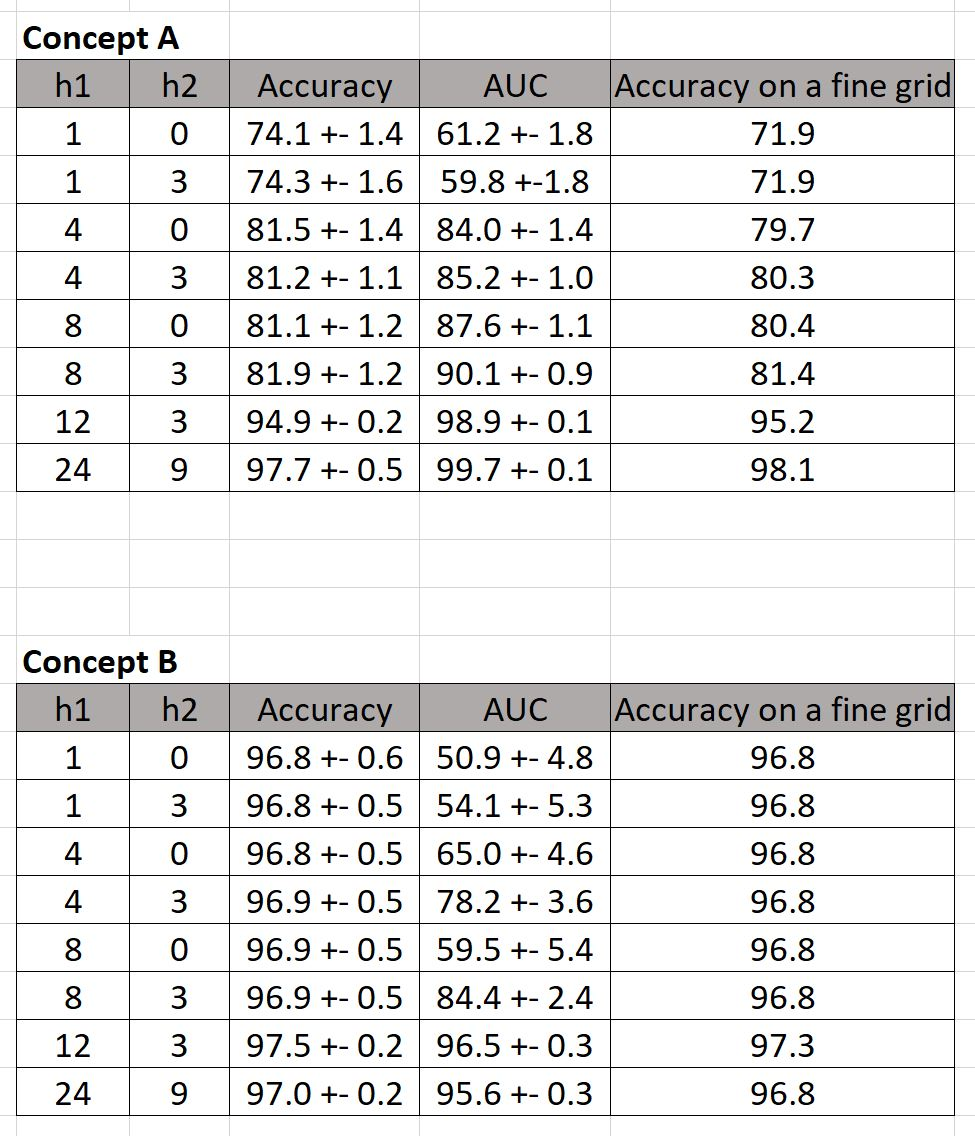
\includegraphics{Q1}

Observations:
\begin{enumerate}
	\item For concept A, in general, the accuracy and AUC keep increasing as we increasing the number of hidden nodes, which is only expected since more hidden nodes can capture more information.
	\item For concept B, the accuracy remain almost the same for most models, this is because the data contains very less examples of the positive class, and hence just classifying all examples as negative gives really high accuracy. This can also be verified from the heat maps which are almost completely black (had the max heat been forced to be equal to 1) in most of the cases. The AUC would change randomly according to the number of positive class points chosen in the validation data, and their prediction, hence the unpredictable AUC pattern with really high standard error.
	\item For some cases we can see that the accuracy calculated on the fine grid is within the 68\% confidence interval, and for some it is not. In theory it should be within the confidence interval for 68\% of the cases but this data was calculated totally randomly and is a very small set of results to be able to verify that.
	\item From the heat maps and from the accuracy on the fine grid we can see that the models with h1=12, h2=3 and h1=24, h2=9, perform really well on both the concepts. Though there isn't much improvement, if there even is improvement at all, of the model with h1=24, h2=9 over the model with h1=12, h2=3. This is because the latter has enough hidden nodes to capture all the information. The 12 nodes in the first layer can linearly separate the space at all the 12 edges, 4 for each of the 3 squares, and then the 3 nodes of the next layer help in identifying if a point belongs to either of the 3 squares. Another interpretation of the 3 nodes of the second layer can be that the 3 nodes help in identifying 3 squares out of all the possible regions that the linear separations of the previous layer produce.
\end{enumerate}

Heat maps for concept A: (but the max heat isn't forced to be 1(just the color can be a bit misleading, so look at the scale on the right))

\begin{tabular}{ cc } 
	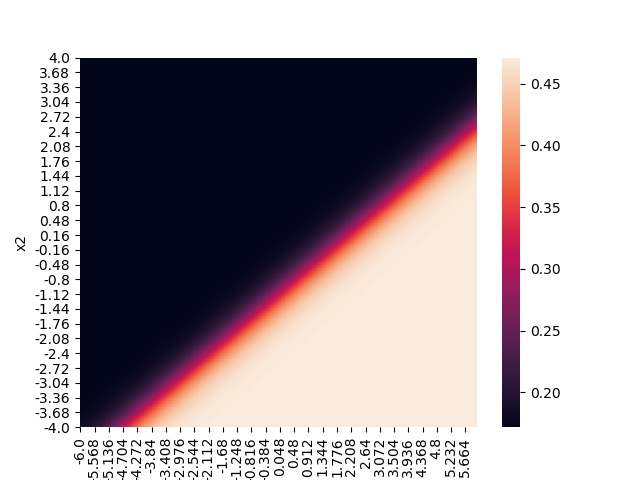
\includegraphics[scale=0.5]{heatmaps1/A1_0} & 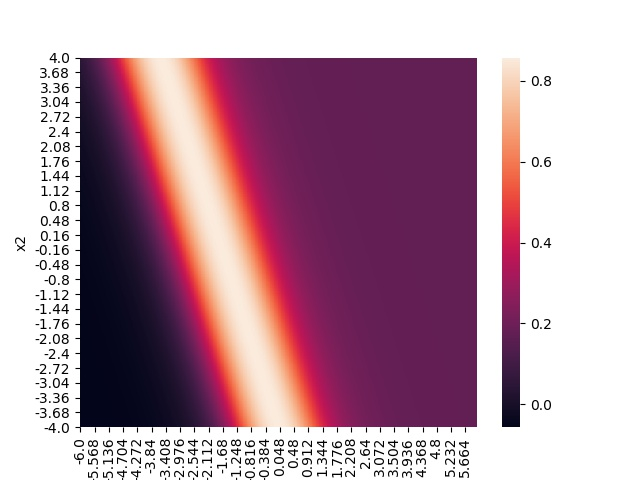
\includegraphics[scale=0.5]{heatmaps1/A1_3} \\ 
	h1=1, h2=0 & h1=1, h2=3 \\ 
	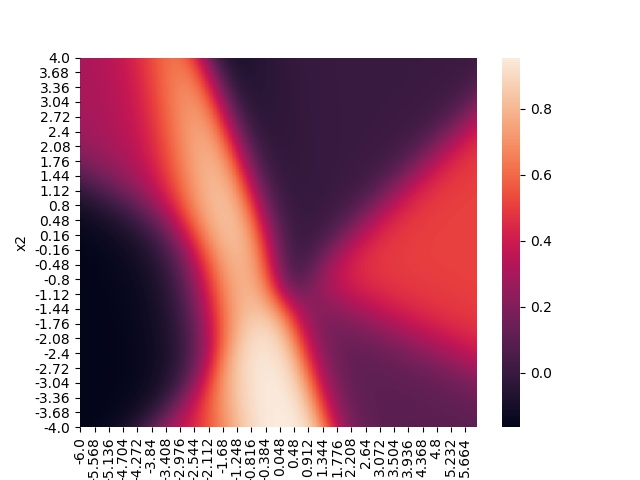
\includegraphics[scale=0.5]{heatmaps1/A4_0} & 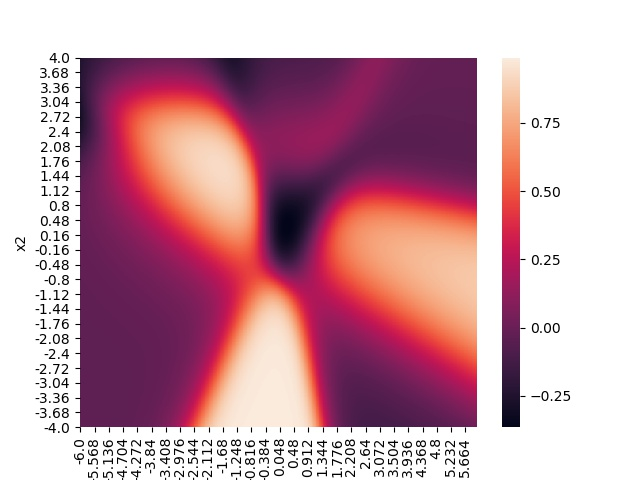
\includegraphics[scale=0.5]{heatmaps1/A4_3} \\ 
	h1=4, h2=0 & h1=4, h2=3 \\ 
\end{tabular}


\begin{tabular}{ cc } 
	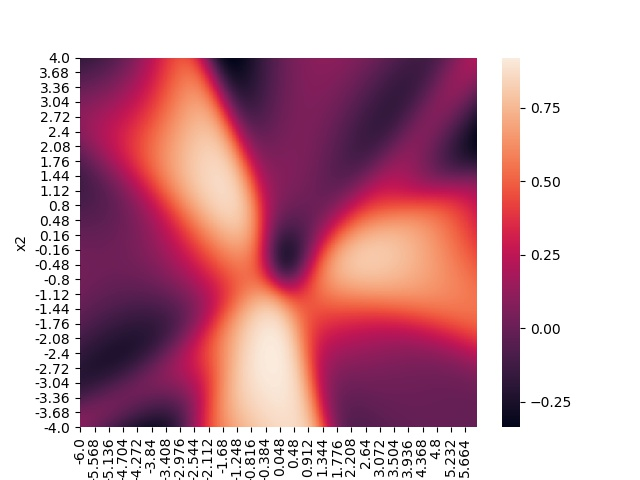
\includegraphics[scale=0.5]{heatmaps1/A8_0} & 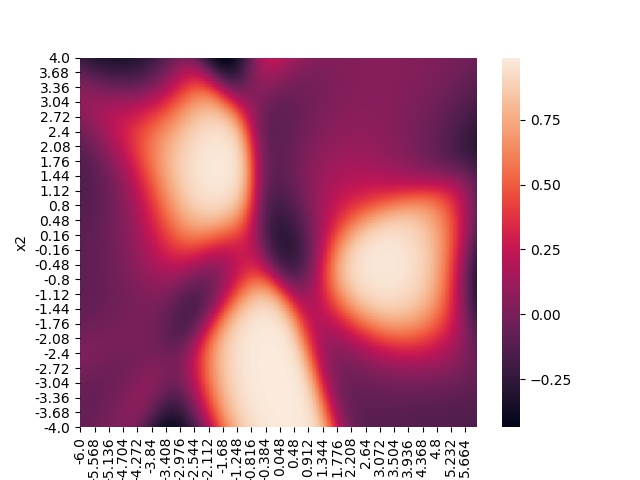
\includegraphics[scale=0.5]{heatmaps1/A8_3} \\ 
	h1=8, h2=0 & h1=8, h2=3 \\ 
	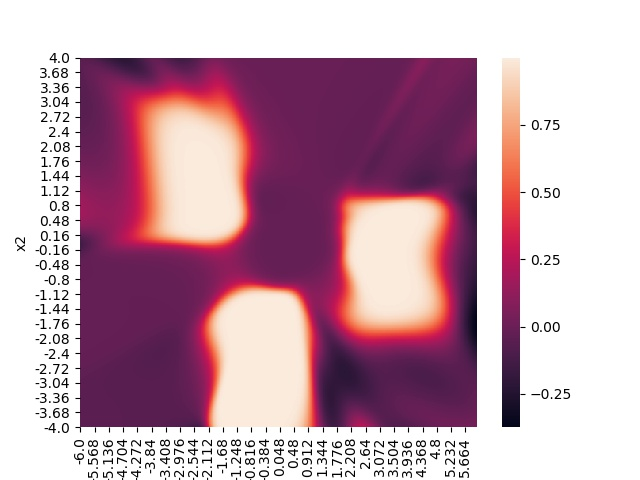
\includegraphics[scale=0.5]{heatmaps1/A1c_12_3} & 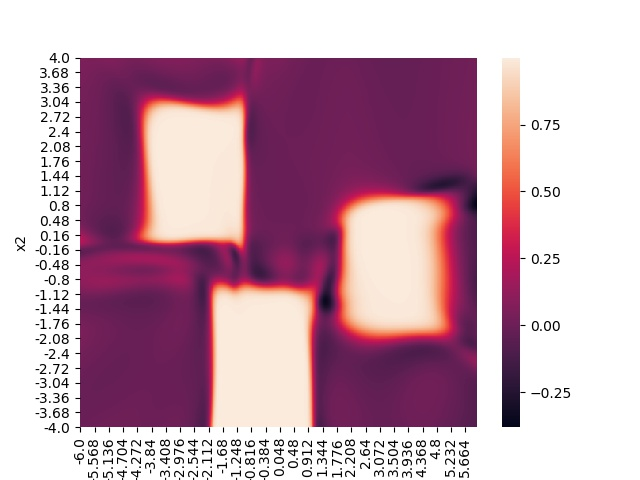
\includegraphics[scale=0.5]{heatmaps1/A1c_24_9} \\ 
	h1=12, h2=3 & h1=24, h2=9 \\ 
\end{tabular}

Heat maps for concept B: (but the max heat isn't forced to be 1(the color can be a bit misleading, so look at the scale on the right), because that just results in almost completely black heat maps.)\\

\begin{tabular}{ cc } 
	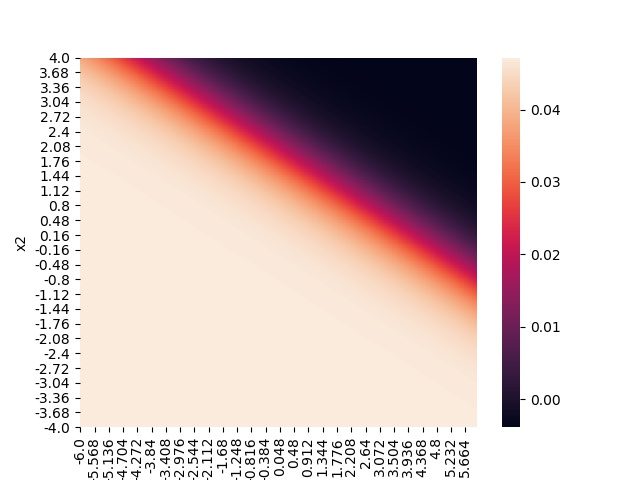
\includegraphics[scale=0.5]{heatmaps1/B1_0} & 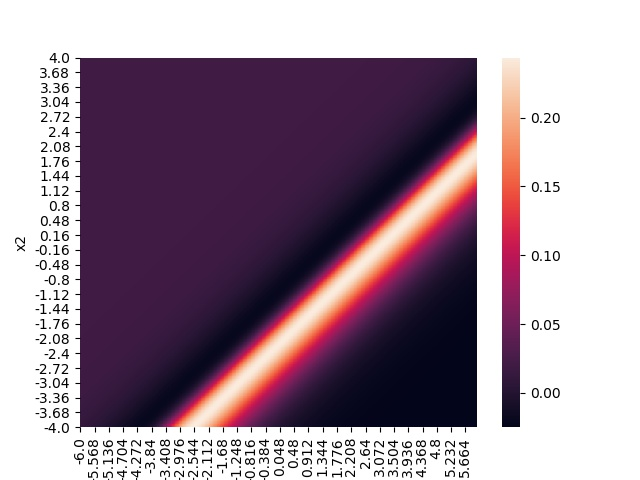
\includegraphics[scale=0.5]{heatmaps1/B1_3} \\ 
	h1=1, h2=0 & h1=1, h2=3 \\ 
\end{tabular}


\begin{tabular}{ cc } 
	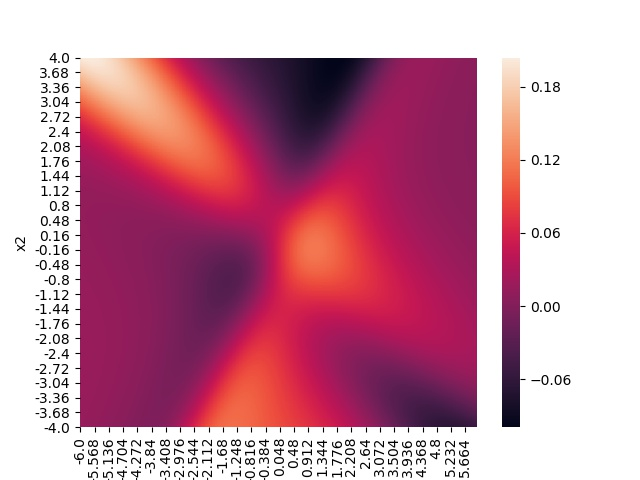
\includegraphics[scale=0.5]{heatmaps1/B4_0} & 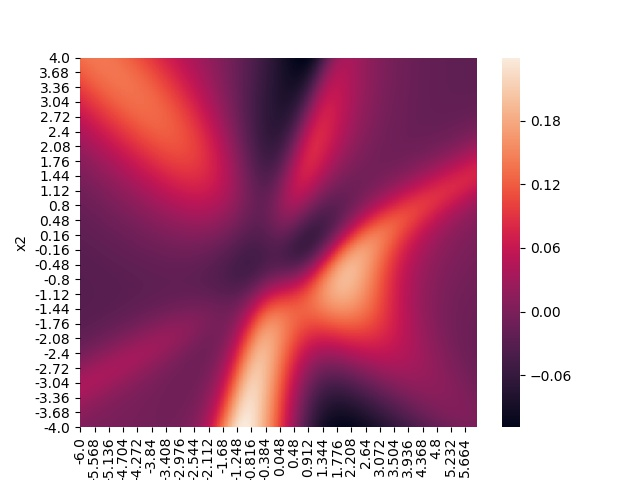
\includegraphics[scale=0.5]{heatmaps1/B4_3} \\ 
	h1=4, h2=0 & h1=4, h2=3 \\ 
	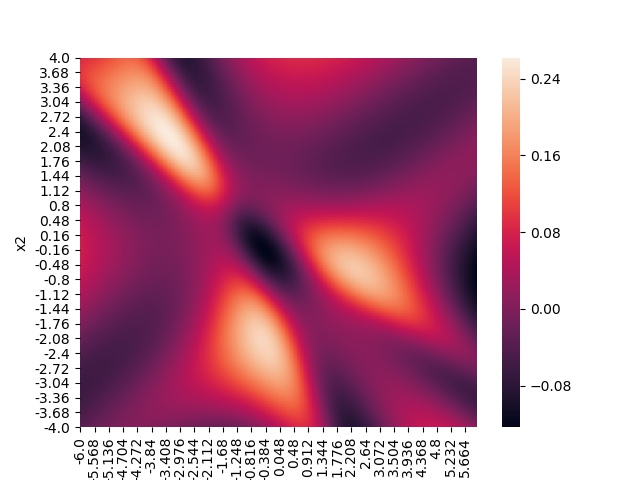
\includegraphics[scale=0.5]{heatmaps1/B8_0} & 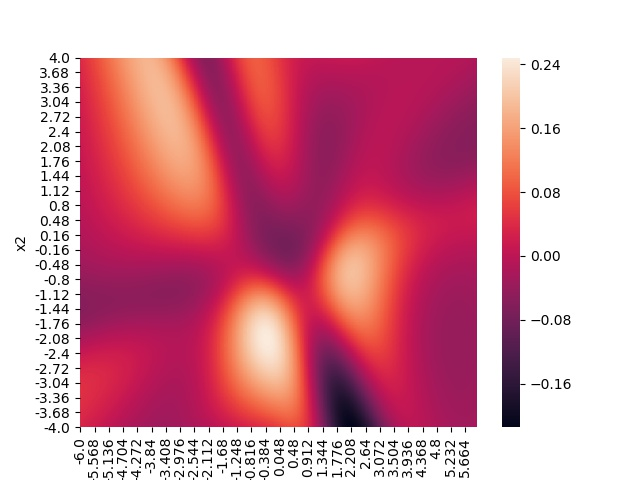
\includegraphics[scale=0.5]{heatmaps1/B8_3} \\ 
	h1=8, h2=0 & h1=8, h2=3 \\ 
	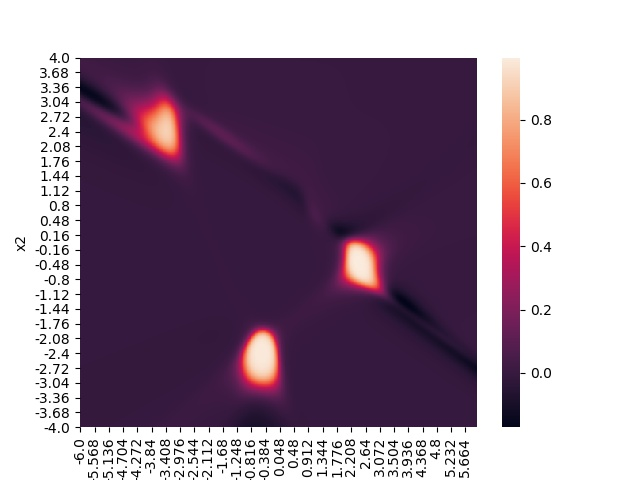
\includegraphics[scale=0.5]{heatmaps1/B1c_12_3} & 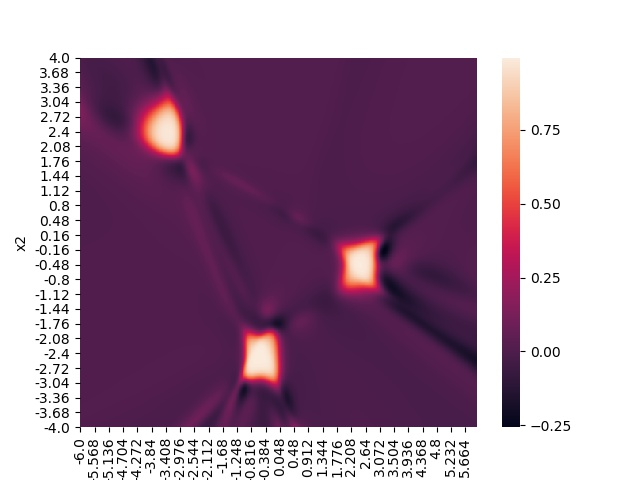
\includegraphics[scale=0.5]{heatmaps1/B1c_24_9} \\ 
	h1=12, h2=3 & h1=24, h2=9 \\ 
\end{tabular}


\pagebreak

%%
%% Problem
%%

\textbf{Problem 2.} (30 points) Repeat step a) from Problem 1 in the following two scenarios.

\begin{enumerate}
\item (10 points) Train 30 neural networks on each data set for each parameter combination. To ensure these 30 trained models are different from one another, you can initialize the weights differently, randomize the order of points fed during the optimization, change training algorithm, etc. To make a prediction on a previously unseen example, average the outputs of 30 models. Report the performance in two tables as before. If computational resources are a problem, use 10 networks as your ensemble and select a subset of parameter combinations such that the computation is feasible.
\item (10 points) Train 30 neural networks, but in each case first sample the training examples with replacement from the original training set (make sure you keep the size of the training set the same as the original training set). Then average the outputs of 30 networks to make predictions on previously unseen examples. Report the performance in two tables as before.
\item (10 points) Discuss your observations from the previous two steps, making sure that you provide plausible explanations for the observed phenomena. Compare both 30-model ensembles to a single model but also two different types of model averaging.
\end{enumerate}

\textbf{Solution}

The following table contains the results (only 10 neural networks were used instead of 30, due to computational limitations):

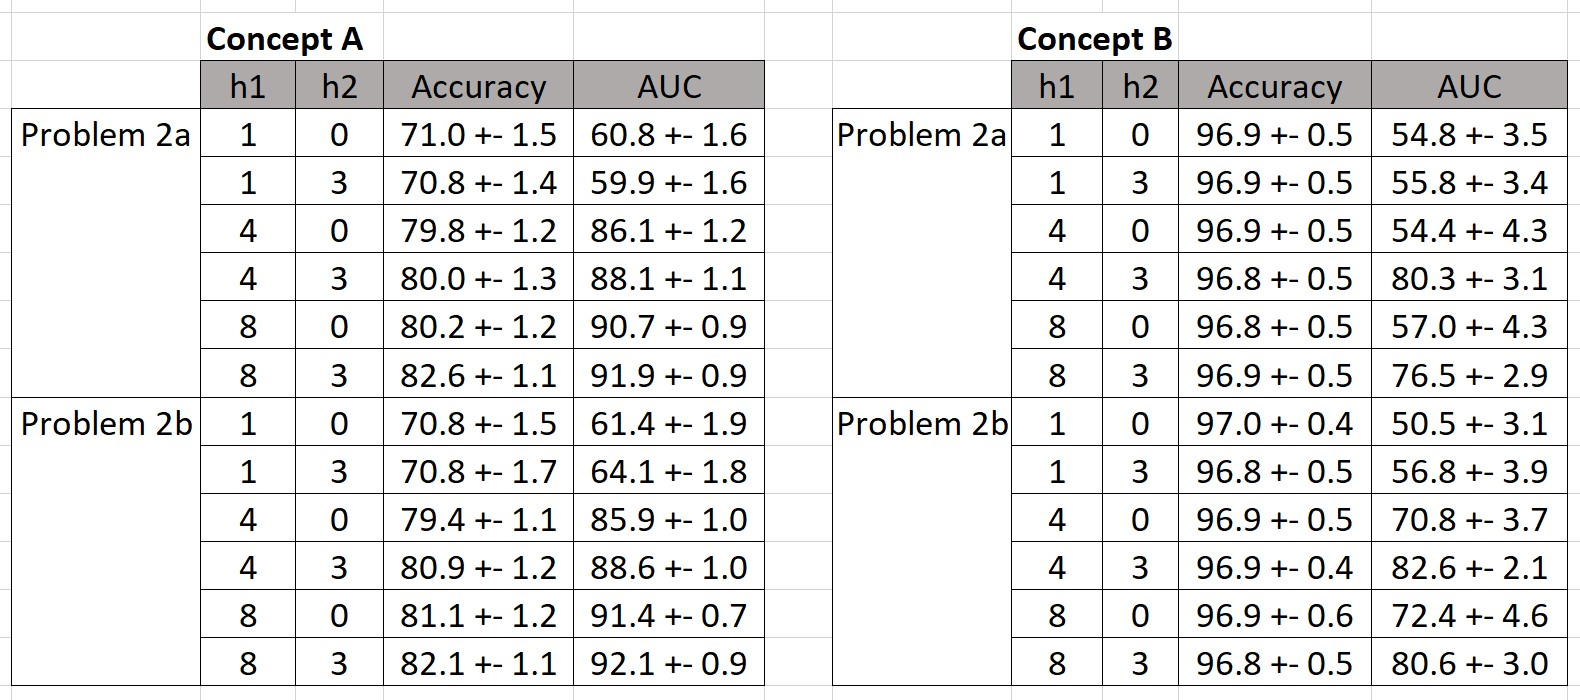
\includegraphics{Q2}

Observations:
\begin{enumerate}
	\item Comparing Q1 to Q2: We can see that there's an improvement when using the ensemble of 10 neural networks even though it is slight, when compared to a single neural network. This is because we're now using the average of 10 models to predict something instead of 1 model. So even if a few of the models misclassify an example but the rest classify it correctly, the overall classification would be correct. Ensemble models are supposed to perform better in theory as well.\\
	\item Comparing the Q2a to Q2b: We can also see that there's some minor improvement in the results (especially the auc) when we are training with sampled examples, in some cases, otherwise it both the methods give somewhat the same results. This may be because the number of ensemble models (10) is too less to show us any difference between the two methods, or that the data concepts are too simple to have any benefit from bagging and all the models are already able to learn the concept well.
	\item Comparing the Q2a to Q2b: Before running the models it was expected that the model with bagging (i.e. the method of training in part b) should show some slight improvement, as it would result different final weights of all the models in the ensemble. But even in part a we initialized the weights of all the models randomly so, even those models would be expected to have different final weights. That may also be the reason why both the methods give similar results.
\end{enumerate}

%%
%% Problem
%%

\textbf{Extra Problem} (15 points) Prove representational equivalence of a three-layer neural network with linear activation function in all neurons and a single-layer layer neural network with the same activation function.

\textbf{Solution}

Approach: I'll be proving this in the case of one hidden layer and show that it recursively holds true for any number of hidden layers.

Let $A, \phi_1, B, \phi_2$ denote the weights and activation functions from the input layer to the first hidden layer and from the first hidden layer to the output layer, respectively. Therefore an input example $x$ would be used to produce an output as follows: $y = \phi_2 (B \phi_1 (Ax))$.
 
A linear function $f$ can be expressed as $f(x) = Cx$, where $C$ is contains coefficients corresponding to all the dimensions of $x$. Note that there is no constant term since we're assuming that we've added $x_0 = 1$ to the vector $x$.

Now since the activation functions are linear they can be rewritten as $\phi_1 = C_1x$ and $\phi_2 = C_2x$. Therefore $y$ can be rewritten as $y = C_2 (B C_1 (Ax))$ or $y = C'x$, since all the matrices can be just combined into one. This is the same as if the neural network just had one layer with the weights $C'$.

It can be easily seen that even if there were $k > 1$ layers all the $\phi$s and the weights could similarly be combined into a single matrix $C'$ and hence be reduced to a single layered neural network.

\end{document}
